\documentclass{article} % say
\usepackage{tikz}
\begin{document}


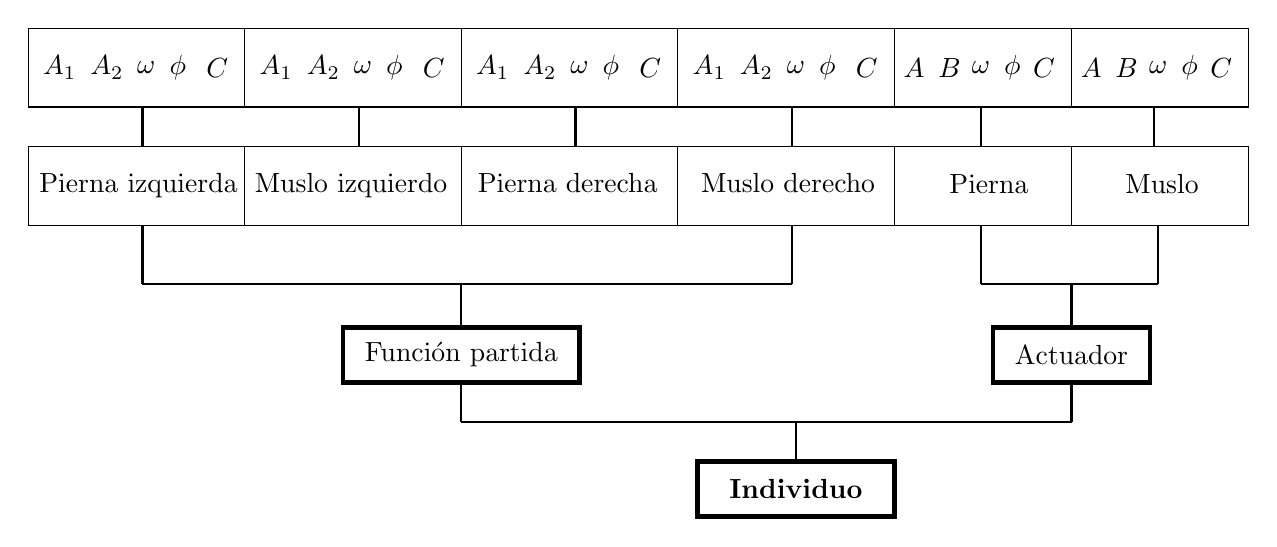
\begin{tikzpicture}
\def\rectanglepath[#1][#2]{-- ++(#1,0cm) -- ++(0cm,#2) -- ++(-#1,0cm) -- cycle}

\draw (6.75,-2.85) node[font=\bf, ultra thick]{Individuo};
\draw[thick] (6.75,-2) -- ++(0cm,-0.5cm) ;
\draw[ultra thick] (5.5,-3.2) \rectanglepath[2.5cm][0.7cm];
\draw[thick] (2.5,-2) -- ++(7.75cm,0cm) ;


\draw (2.5,-1.15) node{Funci\'on partida};
\draw[ultra thick] (1,-1.5) \rectanglepath[3cm][0.7cm];
\draw[thick] (2.5,-1.5) -- ++(0cm,-0.5cm) ;
\draw[thick] (2.5,-0.8) -- ++(0cm,0.55cm) ;
\draw[thick] (-1.55,-0.25) -- ++(8.25cm,0cm) ;


\draw (10.25,-1.15) node{Actuador};
\draw[ultra thick]  (9.25,-1.5) \rectanglepath[2cm][0.7cm];
\draw[thick] (10.25,-1.5) -- ++(0cm,-0.5cm) ;
\draw[thick] (10.25,-0.8) -- ++(0cm,0.55cm) ;
\draw[thick] (9.1,-0.25) -- ++(2.25cm,0cm) ;


\draw (-3,0.5) \rectanglepath[2.75cm][1cm];
\draw (-1.6,1) node{Pierna izquierda};
\draw[thick] (-1.55,0.5) -- ++(0cm,-0.75cm) ;

\draw (-3,2) \rectanglepath[2.75cm][1cm];
\draw (-2.6,2.5) node{$A_1$};
\draw (-2,2.5) node{$A_2$};
\draw (-1.5,2.5) node{$\omega$};
\draw (-1.1,2.5) node{$\phi$};
\draw (-0.6,2.5) node{$C$};
\draw[thick] (-1.55,2) -- ++(0cm,-0.5cm) ;


\draw (-0.25,0.5) \rectanglepath[2.75cm][1cm];
\draw (1.1,1.0) node{Muslo izquierdo};

\draw (-0.25,2) \rectanglepath[2.75cm][1cm];
\draw (0.15,2.5) node{$A_1$};
\draw (0.75,2.5) node{$A_2$};
\draw (1.25,2.5) node{$\omega$};
\draw (1.65,2.5) node{$\phi$};
\draw (2.15,2.5) node{$C$};
\draw[thick] (1.2,2) -- ++(0cm,-0.5cm) ;


\draw (2.5,0.5) \rectanglepath[2.75cm][1cm];
\draw (3.85,1.03) node{Pierna derecha};

\draw (2.5,2) \rectanglepath[2.75cm][1cm];
\draw (2.9,2.5) node{$A_1$};
\draw (3.5,2.5) node{$A_2$};
\draw (4.0,2.5) node{$\omega$};
\draw (4.4,2.5) node{$\phi$};
\draw (4.9,2.5) node{$C$};
\draw[thick] (3.95,2) -- ++(0cm,-0.5cm) ;


\draw (5.25,0.5) \rectanglepath[2.75cm][1cm];
\draw (6.65,1.03) node{Muslo derecho};
\draw[thick] (6.7,0.5) -- ++(0cm,-0.75cm) ;

\draw (5.25,2) \rectanglepath[2.75cm][1cm];
\draw (5.65,2.5) node{$A_1$};
\draw (6.25,2.5) node{$A_2$};
\draw (6.75,2.5) node{$\omega$};
\draw (7.15,2.5) node{$\phi$};
\draw (7.65,2.5) node{$C$};
\draw[thick] (6.7,2) -- ++(0cm,-0.5cm) ;


\draw (8,0.5) \rectanglepath[2.25cm][1cm];
\draw (9.2,1.02) node{Pierna};
\draw[thick] (9.1,0.5) -- ++(0cm,-0.75cm) ;

\draw (8,2) \rectanglepath[2.25cm][1cm];
\draw (8.25,2.5) node{$A$};
\draw (8.7,2.5) node{$B$};
\draw (9.1,2.5) node{$\omega$};
\draw (9.5,2.5) node{$\phi$};
\draw (9.9,2.5) node{$C$};
\draw[thick] (9.1,2) -- ++(0cm,-0.5cm) ;


\draw (10.25,0.5) \rectanglepath[2.25cm][1cm];
\draw (11.4,1.02) node{Muslo};
\draw[thick] (11.35,0.5) -- ++(0cm,-0.75cm) ;

\draw (10.25,2) \rectanglepath[2.25cm][1cm];
\draw (10.5,2.5) node{$A$};
\draw (10.95,2.5) node{$B$};
\draw (11.35,2.5) node{$\omega$};
\draw (11.75,2.5) node{$\phi$};
\draw (12.15,2.5) node{$C$};
\draw[thick] (11.3,2) -- ++(0cm,-0.5cm) ;



\end{tikzpicture}



\end{document}